\documentclass[class=book, crop=false, oneside]{standalone}
\usepackage[subpreambles=true]{standalone}

\usepackage{../../style}

\graphicspath{{./assets/images/}}
\newmintinline{asm}{}

% arara: pdflatex: { synctex: yes, shell: yes }
% arara: latexmk: { clean: partial }
%! arara: clean: { extensions: [sta] }
\begin{document}
\chapter{L'architettura MIPS}

Dopo la breve introduzione del precedente capitolo, affronteremo ora lo studio dell'architettura \emph{MIPS}; iniziamo con questa perché, seppur non molto diffusa, è molto simile ad altre architetture che vedremo in seguito (soprattutto ARM), ed è quindi propedeutica.

\section{Breve riepilogo su ISA}
Come sappiamo già, ogni processore possiede un proprio linguaggio macchina, che non è altro che una sorta di "vocabolario di istruzioni" detto \emph{instruction set architecture} (o \emph{ISA} per gli amici); queste istruzioni sono solitamente le operazioni aritmetiche fondamentali (a parte quelle che lavorano su floating point) e quelle logiche.\\
Nonostante ogni processore possieda un proprio ISA, le differenze non sono poi così grandi (motivo per cui conoscere MIPS ci agevolerà molto nell'apprendimento di altre ISA); una similitudine adeguata può essere fatta con i dialetti di una lingua maggiore (per esempio, veneziano, trevigiano e veronese sono tutte varianti locali mutualmente intelligibili della Grande Lingua Veneta).

Lo scopo di avere questi sistemi di istruzioni è poter controllare e sfruttare la potenza di calcolo fornita dai nostri calcolatori senza conoscerne i dettagli; inoltre, come già fatto notare da Von Neumann nel 1947, la progettazione di un'architettura influisce enormemente sull'efficienza dell'hardware, ed è quindi fondamentale che si ricerchino istruzioni \emph{semplici, chiare e veloci}.

Un organico di istruzioni andrà a costruire un \emph{programma memorizzato} che, come approfondiremo, altro non è che un insieme di istruzioni mappato sotto forma di numero binario, non diversamente da numeri o qualsiasi altro dato.

\subsubsection{Cos'è MIPS}
Come già detto, nonostante non sia diffusissima, inizieremo a studiare l'architettura MIPS in quanto propedeutica. È una cosiddetta architettura \emph{RISC} "pragmatica", ossia un'architettura ibrida la quale, pur essendo basata su \emph{RISC} e quindi con un numero limitato di istruzioni disponibili, possiede anche alcune operazioni complesse tipiche delle ISA \emph{CISC}.\\
Per quanto semplice e vicino al linguaggio macchina un linguaggio potesse essere, era chiaro fin dai tempi di Von Neumann che non dovevano mancare le operazioni aritmetiche e logiche fondamentali; oltre a quelle, MIPS possiede inoltre alcuni comandi per il controllo di flusso.

\section{Operazioni aritmetiche}
Per dare una chiave di lettura al percorso che faremo su MIPS useremo alcuni principi di progettazione software e hardware che ogni informatico segue fin dagli albori, e naturalmente, introducendo le operazioni aritmetiche, inizieremo così:

\vspace{8pt}
\begin{tcolorbox}
\centering
\textbf{Primo principio di progettazione}\\
\emph{La semplicità favorisce la regolarità}.
\end{tcolorbox}
\vspace{5pt}

In linea con questo principio, MIPS consente di effettuare operazioni aritmetiche solo nella loro forma più semplice, ossia con tre operandi: \mintinline{c}{a = b + c}.
Quest'istruzione, comune in C, Java, Python o altri linguaggi, in MIPS sarà scritta così:
\begin{minted}[linenos]{asm}
add a, b, c
\end{minted}

Notiamo subito che l'operando "di destinazione" viene messo come primo elemento (in altre ISA non è sempre così, tuttavia).\\
Naturalmente, mentre nei linguaggi ad alto livello possiamo agevolmente scrivere espressioni matematiche complesse, in MIPS verranno tutte mappate in espressioni semplici, sicché una linea di codice come \mintinline{c}{f = (g + h) - (i + j)}, per quanto banale, può essere srotolata in diverse righe assembly:

\begin{minted}[linenos]{asm}
add t0, g, h   # t0 (variabile temp) = g + h
add t1, i, j   # t1 (variabile temp) = i + j
sub f, t0, t1  # f = t0 - t1
\end{minted}

La sintassi per scrivere commenti consiste nell'anteporre un \# al testo che si vuole inserire. Come per // in C, anche \# agisce solo su una riga.

Esistono però alcune eccezioni: ad esempio \mintinline{batch}{gcc}, l'assembler di Unix, usa i commenti come il C e l'operando di destinazione delle operazioni va in fondo.

\section{I registri}

\subsection*{Cosa sono}

Fino ad ora abbiamo considerato gli operandi come fossero normali variabili, ma in realtà questi altro non sono che dei \emph{registri}, ossia delle particolari locazioni di memoria interne al processore che possono essere reperite molto rapidamente, in un solo colpo di clock.\\

MIPS possiede 32 registri, ciascuno di 32 bit, per cui ogniqualvolta si debba eseguire delle operazioni è necessario caricare i dati dalla RAM con un'operazione di \emph{load}. Questo processo può apparire dispendioso ed è lecito domandarsi come mai non ci si possa dotare di più registri più capienti, e la risposta è espressa dal secondo principio di progettazione.

\vspace{8pt}
\begin{tcolorbox}
\centering
\textbf{Secondo principio di progettazione}\\
\emph{Minori sono le dimensioni, maggiore è la velocità}.
\end{tcolorbox}
\vspace{5pt}

Di fatto, se avessimo  più registri, aumenterebbe notevolmente il tempo di accesso a questi, in quanto gli impulsi elettrici impiegherebbero fisicamente più tempo per passare da un registro all'altro, e la velocità di clock sarebbe sensibilmente compromessa.

\subsection*{Gestione dei registri}

\paragraph{Notazione}
A questo punto, tornando all'esempio in 1.2, illustriamo la sintassi per richiamare un registro:
\begin{minted}[linenos, breaklines]{asm}
add $t0, $s1, $s2  # al registro temporaneo t0 viene assegnato il valore come somma di s1 + s2
add $t1, $s3, $s4  # come prima
sub $s0, $t0, $t1  # f = t0 - t1
\end{minted}
Come si evince, è sufficiente anteporre un \$ al nome del registro.

\subsubsection{Movimenti}
Naturalmente, i registri non sono minimamente sufficienti per contenere tutti i dati di un programma complesso (soprattutto perché alcuni vengono usati dal kernel e dal sistema operativo), ma le operazioni possono essere eseguite solo fra registri. Diventa quindi necessaria l'implementazione delle funzioni \emph{load} che, come anticipato, carica i dati dalla RAM a un registro, e \emph{store}, che passa il dato dal registro alla RAM.

La memoria è solitamente organizzata in gruppi da 8 bit (ossia 1 byte) ciascuno associato ad  un indirizzo lineare progressivo, ma il prelievo e il salvataggio dei dati segue un cosiddetto \emph{vincolo di allineamento}: viene fissato un \emph{offset} (\emph{spiazzamento}) di 4 byte (quindi della stessa dimensione dei registri), dimodoché ogni informazione che passa abbia la medesima dimensione di un registro (anche il program counter viene incrementato di 4 byte ogni fetch) e sia possibile accedere solamente ad indirizzi multipli di 4 byte. In questo contesto, ogni informazione di 4 byte che viene spostata tra RAM e registri viene detta \emph{parola}.\\
L'indirizzo di ogni parola viene quindi espresso con una \emph{base}, specifica per registro, e con lo \emph{spiazzamento} costante di cui abbiamo parlato prima.

\paragraph{Load and store}
Ecco un esempio di istruzione di load (analogamente per la store):
\begin{figure}[H]
	\centering
	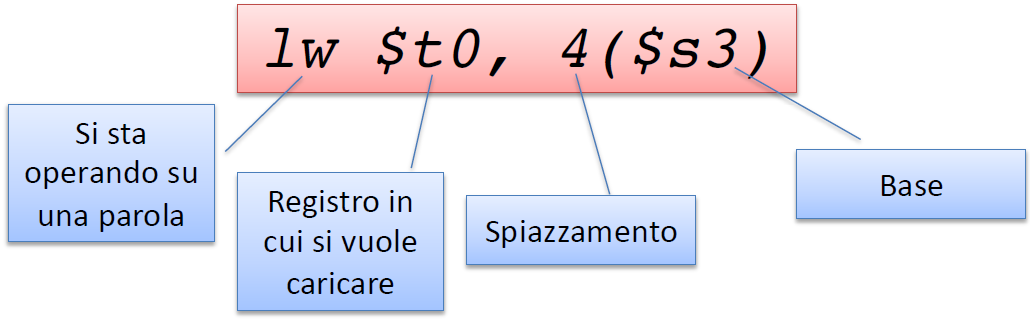
\includegraphics[width=0.7\textwidth,keepaspectratio]{load}
	\caption{Descrizione di una load}
\end{figure}
Adesso prendiamo invece una semplice riga di codice:
\begin{minted}[linenos]{c}
A[12] = h + A[8];
\end{minted}
E vediamone ora la traduzione fatta dal compilatore:
\begin{minted}[linenos, breaklines]{asm}
lw $t0, 32($s3)   # la parola 8 comincia all'indirizzo 32(=8*4) e il puntatore A è in $s3
add $t0, $s2, $t0 # h è in $s2
sw $t0, 48($s3)   # memorizzo il contenuto di $t0 in A[12]
\end{minted}

\paragraph{Register Spilling}
Come già anticipato, i 32 registri non sono assolutamente sufficienti per contenere tutte le variabili usate da un programma complesso. Quello che succede a livello assembly, eseguito dal compilatore, è un continuo susseguirsi di load e store chiamato \emph{register spilling} (si dice che prepara il \emph{working set}, ossia una stima delle load e store appropriate).

\subsection*{Le costanti}
Molto spesso ci si trova a lavorare con le costanti. Nonostante ogni costante possa essere salvata su un registro, questa soluzione è parecchio inefficiente, perché le costanti e le operazioni relative sono molto comuni.

\vspace{8pt}
\begin{tcolorbox}
\centering
\textbf{Terzo principio di progettazione}\\
\emph{Rendi più veloci possibile le operazioni comuni}.
\end{tcolorbox}
\vspace{5pt}

Quindi ci conviene assolutamente costruire una sintassi dedicata all'esecuzione di operazioni con costanti, dove la \emph{i} sta per \emph{immediate}. Ad esempio \mintinline{c}{f = f + 4} diventa: \mintinline{asm}{addi $s3, $s3, 4}.

Per dare un altro esempio, è molto conveniente implementare un registro zero (\emph{\$zero}), perché rende molto più semplici le operazioni di copia, che di fatto possono essere ridotte a una somma di un qualsiasi registro con il registro zero.

\section{La rappresentazione delle istruzioni}

\subsubsection{Convenzioni sulla scrittura esadecimale}
Prima di indicare come vengono codificate le istruzioni, ricordiamo che 1 byte è agevolmente rappresentabile con due cifre esadecimali (essendo composto da 8 bit e sapendo che ogni cifra esadecimale corrisponde a 4 bit). Ad esempio, \(1001 1101_{2}\) diventa \(9D_{16}\). Inoltre, quando si scrive in esadecimale, si usa di solito precedere la scrittura con \emph{0x}. Ad esempio: \emph{0xEA01BD1C}.

Quando si devono codificare parole di 4 byte è importante decidere dove vada il byte più significativo:
\begin{itemize}[nolistsep]
	\item se il byte più significativo è posto per primo, la notazione è detta \emph{big endian} (usata nei processori Motorola e protocolli internet).
	\item se il byte meno significativo è posto per primo, la notazione è detta \emph{little endian} (usata nei processori Intel).
\end{itemize}

\subsection{Le istruzioni register}\label{subsec:campiIstruzione}
Come anticipato, le istruzioni vengono codificate come numeri binari. In particolare, ogni istruzione dovrà essere mappata utilizzando parole di soli 32 bit, ma come viene impostato questo processo?\\
Prendiamo come esempio l'istruzione di somma \mintinline{asm}{add $t0, $s1, $s2}: avremo bisogno di un codice per l'istruzione di somma e uno per ogni registro; l'operazione sarà scritta nei primi 6 bit e negli ultimi 6, mentre i 20 in bit in mezzo saranno divisi in gruppi da 5 bit ciascuno: i primi tre gruppi ospiteranno i registri, e l'ultimo sarà usato per comandi speciali (come lo shift, che vedremo in seguito).
\begin{figure}[H]
	\centering
	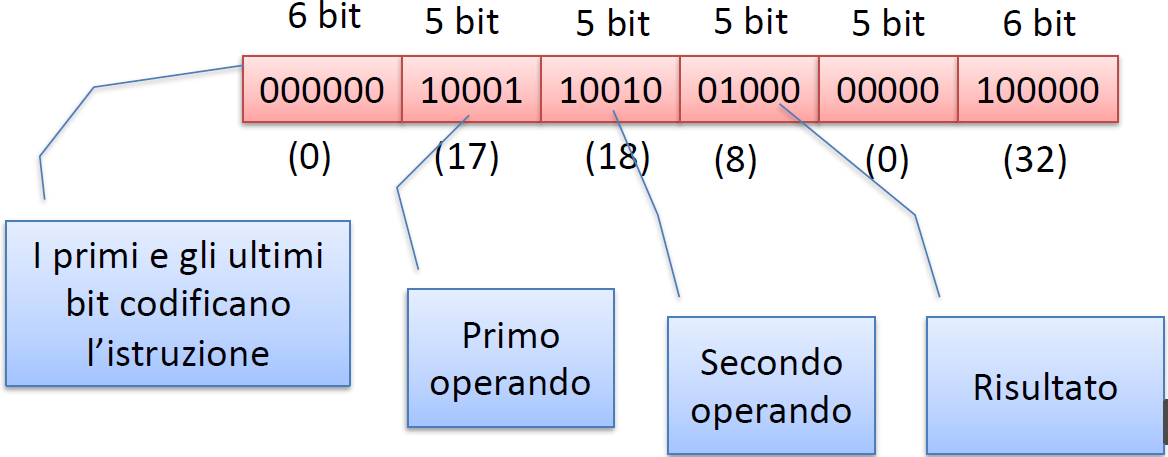
\includegraphics[width=0.8\textwidth,keepaspectratio]{istruzioni.png}
	\caption{Esempio di somma}
\end{figure}
In generale questo sistema, detto R (da registro), ogni campo dell'istruzione ha un nome:
\begin{itemize}[noitemsep]
	\item \emph{op}: codice operativo dell'istruzione.
	\item \emph{rs}: primo operando sorgente.
	\item \emph{rt}: secondo operando sorgente.
	\item \emph{rd}: operando di destinazione.
	\item \emph{shamt}: shift amount (specifico per alcune istruzioni).
	\item \emph{funct}: definisce la funzionalità specifica dell'istruzione (insieme ad op). Ad esempio la sottrazione è un particolare tipo di addizione.
\end{itemize}

\begin{figure}[H]
	\centering
	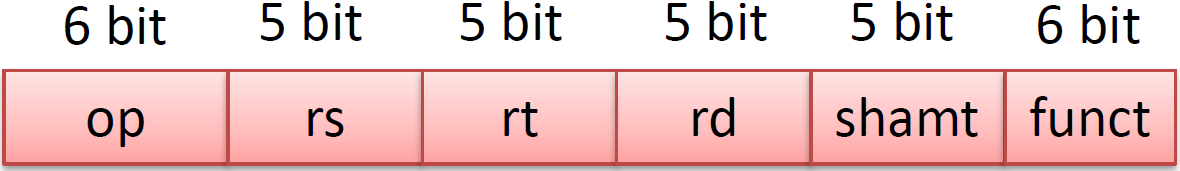
\includegraphics[width=0.7\textwidth,keepaspectratio]{mappatura.png}
\end{figure}

A questo punto è lecito domandarsi come mai si usino solo 32 bit per rappresentare le istruzioni. La risposta si trova nel quarto principio di progettazione.

\vspace{8pt}
\begin{tcolorbox}
\centering
\textbf{Quarto principio di progettazione}\\
\emph{Un buon progetto richiede buoni compromessi}.
\end{tcolorbox}
\vspace{5pt}

Utilizzando una quantità limitata di registri e istruzioni, è dunque possibile guadagnare moltissimo in efficienza!

\subsection{Le istruzioni immediate}
Nei casi di indirizzamento immediato e di operazioni con costanti, MIPS mette a disposizione una diversa mappatura, detta appunto \emph{I}. Forniamo qui un esempio e invitiamo il lettore a confrontare la seguente mappatura con l'equivalente R.
\begin{figure}[H]
	\centering
	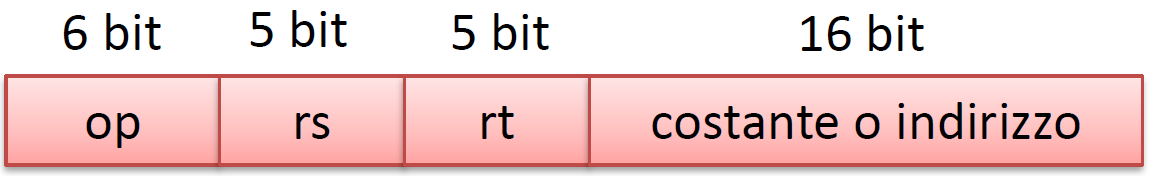
\includegraphics[width=0.7\textwidth,keepaspectratio]{I.png}
	\caption{Mappatura di un'istruzione I}
\end{figure}

Prendiamo come esempio la riga di codice \mintinline{c}{A[300] = h + A[300]}. Essa verrà tradotta in MIPS come:
\begin{minted}[linenos]{asm}
lw $t0, 1200($t1)
add $t0, $s2, $t0
sw $t0, 1200($t1)
\end{minted}
Osserviamo nel dettaglio cosa succede:
\begin{figure}[H]
	\centering
	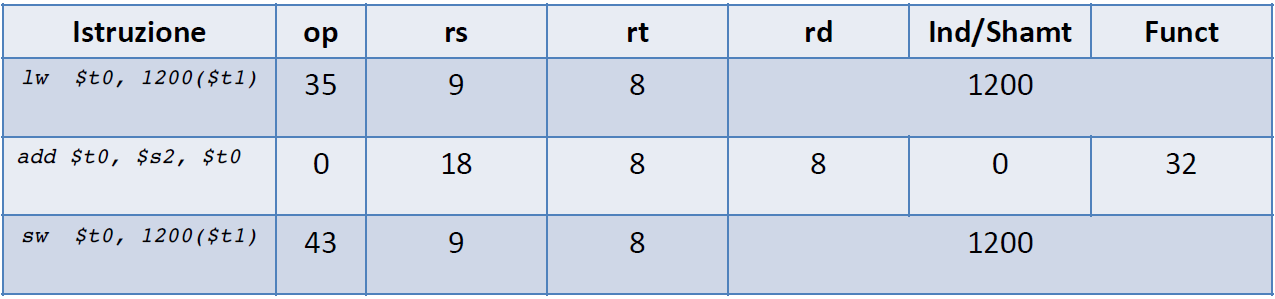
\includegraphics[width=1\textwidth,keepaspectratio]{nat.png}
\end{figure}
\begin{figure}[H]
	\centering
	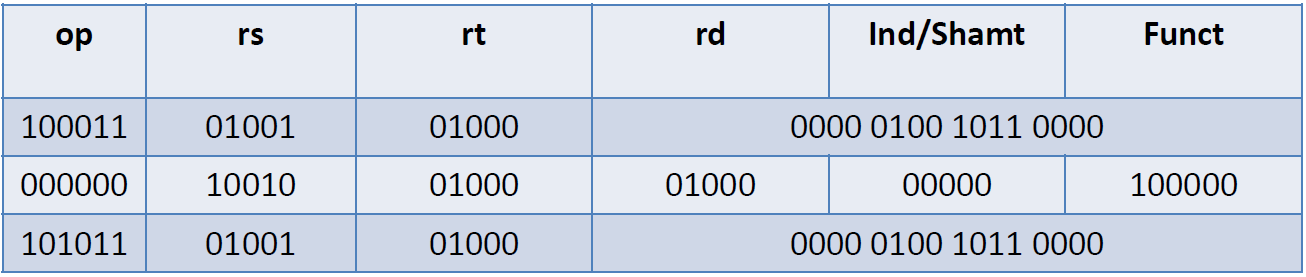
\includegraphics[width=1\textwidth,keepaspectratio]{bin.png}
	\caption{Trascrizione del codice sopra riportato, prima in decimale e poi in binario}
\end{figure}

\section{Istruzioni aritmetico-logiche}

Inizialmente i calcolatori erano capaci di operare unicamente su parole intere, ma ben presto si manifestò la necessità di andare ad agire solo su determinate porzioni di parole, o anche sui singoli bit. A seguire presenteremo alcune delle istruzioni che MIPS mette a disposizione qualora si presentasse la suddetta situazione.

\subsection{Operazioni di shift}

\paragraph{Shift logico a sinistra}
Consideriamo lo \emph{shift logico a sinistra}: l'idea consiste nell'inserire degli zeri nella posizione meno significativa e traslare tutto a sinistra perdendo, nel caso di overflow, i bit più significativi.

\begin{minted}[linenos, breaklines]{asm}
sll $t2, $s0, 4  # memorizza in t2 il contenuto del registro s0 shiftato a sinistra di 4
\end{minted}

Lo shift massimo che è possibile eseguire è di 32 bit (infatti, come precedentemente visto, vengono allocati 5 bit per il campo di \emph{shift amount}). Ciò non risulta un problema in quanto il vincolo di allineamento definito dall'implementazione MIPS che affronteremo è costituito da 32 bit.\\
Eseguire uno shift a sinistra di \(k\) bit di un numero \(n\) positivo, consiste nel moltiplicare \(n\) per \(2^k\). Fanno eccezione solo alcuni casi in cui si lavora con numeri interi codificati in complemento a 2: in questo frangente, si potrebbe uscire dal \emph{range di rappresentazione} del CA2.

\paragraph{Shift logico a destra}
In maniera analoga, lo \emph{shift logico a destra} consiste nell'inserire degli zeri nella posizione più significativa, traslando tutto a destra. Come per lo shift logico a sinistra, anche qui è possibile effettuare uno shift di al massimo 32 bit.

\begin{minted}[linenos, breaklines]{asm}
srl $t2, $s0, 1  # memorizza in t2 il contenuto del registro s0 shiftato logicamente a destra di 1
\end{minted}

Applicare uno shift logico a destra di \(k\) bit ad un numero \(n\) positivo è equivalente a dividere (divisione intera) \(n\) per \(2^k\). Lo shift logico a destra non è utilizzabile in nessun caso con un numero negativo codificato in CA2 (proprio per questo è stato introdotto lo shift aritmetico a destra).

\paragraph{Shift aritmetico a destra}
Dunque, per trovare una soluzione all'implementazione della divisione intera anche per i numeri negativi codificati in CA2, è stato introdotto lo \emph{shift aritmetico a destra}.

\begin{minted}[linenos, breaklines]{asm}
sra $t2, $s0, 1  # memorizza in t2 il contenuto del registro s0 shiftato aritmeticamente a destra di 1
\end{minted}

Piuttosto che inserire 0 come bit più significativo, come avviene nello shift logico, lo shift aritmetico a destra inserisce bit uguali al bit di segno. Dunque risolve i problemi con CA2.\\
Si noti come non abbia senso parlare di shift aritmetico a sinistra, in quanto o il risultato è rappresentabile (attraverso lo shift logico) o non lo è (a causa di un overflow).

\subsection{Operazioni bitwise}
Vengono definite \emph{bitwise} quelle operazioni logiche che operano su ciascun bit.

\paragraph{Bitwise AND}
L'operazione di \emph{bitwise AND} viene applicata principalmente per forzare alcuni bit a 0 usando come operando una maschera (i cui bit corrispondenti a quelli che si vogliono annullare sono settati a 0).
\begin{figure}[H]
	\centering
	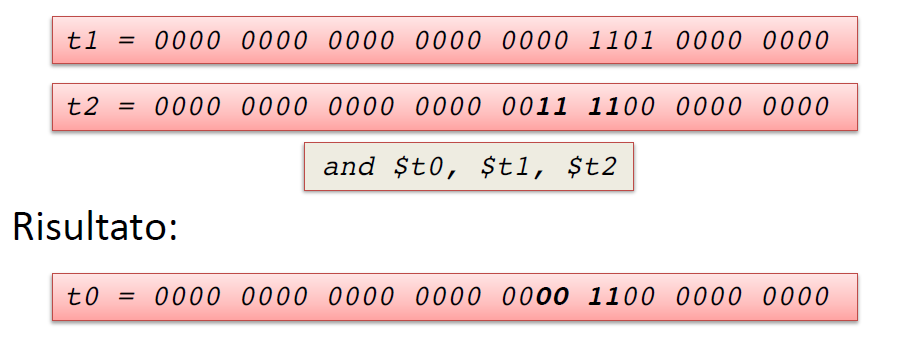
\includegraphics[width=0.7\textwidth,keepaspectratio]{bitwise_and}
	\caption{Funzione "maschera" del bitwise AND}
\end{figure}

\paragraph{Bitwise OR}
In maniera analoga, è possibile settare a \(1\) alcuni bit applicando l'operazione di \emph{bitwise OR} con un operando che abbia \(1\) nella posizione corrispondente (funzione di maschera). Ad esempio, per impostare ad \(1\) i \(4\) bit più significativi di \emph{\$s0}:
\begin{minted}[linenos]{asm}
addi $t0, $zero, 0x000F
sll $t0, $t0, 28
or $s0, $s0, $t0
\end{minted}

Un ulteriore esempio riguarda quello della \emph{rotazione} dei \(4\) bit più significativi di una parola sui suoi bit meno significativi:
\begin{minted}[linenos, breaklines]{asm}
# si ottengono i 4 bit più significativi, spostandoli nei 4 meno significativi di $t0
srl $t0, $s0, 28

# si azzerano i 4 bit più significativi di $s0
sll $s0, $s0, 4
srl $s0, $s0, 4

# operazione di maschera
or $s0, $s0, $t0
\end{minted}

\paragraph{Bitwise NOR}
L'operazione di \emph{NOR} viene definita come segue:
\begin{table}[H]
	\centering
	\subimport{assets/tables/}{nor.tex}
	\caption{Tabella di verità NOR}
\end{table}

A seguire la sintassi MIPS dell'istruzione di \emph{bitwise NOR}:
\begin{minted}[linenos]{asm}
nor $t0, $t1, $t2
\end{minted}

\paragraph{Bitwise NOT}
Dato il fatto che l'operatore di \emph{NOT} è unario, esso non è implementato in MIPS, per non interrompere la regolarità delle istruzioni a tre operandi. Un modo per ottenere il \emph{NOT}, grazie alle leggi di De Morgan, è il seguente:
\begin{minted}[linenos]{asm}
nor $t0, $t1, $zero  # equivale a: not $t1
\end{minted}

\paragraph{OR esclusivo (XOR)}
L'\emph{OR esclusivo} produce \(1\) se i due bit di ingresso sono diversi, altrimenti \(0\) se sono uguali. Segue la tabella di verità:
\begin{table}[H]
	\centering
	\subimport{assets/tables/}{xor.tex}
	\caption{Tabella di verità XOR}
\end{table}

A seguire la sintassi MIPS dell'operazione di \emph{XOR}:
\begin{minted}{asm}
xor $t0, $t1, $t2  # $t0 = $t1 xor $t2
\end{minted}

Curiosità: se si esegue lo \emph{XOR} di un numero con se stesso, il risultato è pari a \(0\) per ciascun bit.

\section{Salti}
Oltre alle istruzioni aritmetico-logiche e di lettura e scrittura in memoria, il linguaggio MIPS offre anche alcune istruzioni per effettuare dei "salti" all'interno del codice. In particolare, si dicono \emph{istruzioni di salto} quei comandi che possono modificare il valore del registro PC.\\
Esistono sostanzialmente due differenti tipi di salto:
\begin{itemize}
	\item \emph{jump}: salto non condizionato.
	\item \emph{branch}: salto condizionato.
\end{itemize}
A differenza delle istruzioni di jump, i branch vengono eseguiti solo se una determinata condizione è verificata: uguaglianza di due registri (nel caso di \mintinline{asm}{beq}) e disuguaglianza di due registri (nel caso di \mintinline{asm}{bne}). Si definiscono perciò come operazioni che hanno la capacità di modificare il flusso del programma.

A seguire la sintassi delle istruzioni di salto offerte da MIPS:
\begin{minted}[linenos, breaklines]{asm}
# Branch Equal
beq reg1, reg2, L1  # vai a L1 se reg1 == reg2

# Branch Not Equal
bne reg1, reg2, L1  # vai a L1 se reg1 != reg2

# Jump
j LABEL  # salta incondizionatamente a LABEL

# Jump Register
jr $t0  # salta incondizionatemente all'indirizzo contenuto nel registro t0
\end{minted}

Come si può osservare, in fase di scrittura del codice si utilizzano delle \emph{label} (ossia etichette) piuttosto che veri e propri indirizzi di memoria. L'arduo compito di tradurre queste etichette in veri e propri indirizzi di memoria spetta al compilatore.

\paragraph*{Blocco di base} Viene data la seguente definizione di \emph{blocco di base}: sequenza di istruzioni che non contiene né istruzioni di salto (con l’eccezione dell’ultima) né etichette di destinazione (con l’eccezione della prima); sostanzialmente, una porzione di codice compresa tra due salti. In fase di compilazione ricoprono un ruolo non indifferente, in quanto una delle prime analisi eseguite sul codice consiste nel cercare proprio queste porzioni di codice. Inoltre, tutti i cicli dei linguaggi di programmazione ad alto livello vengono implementati con l'ausilio di blocchi base.

\subsection*{Confronti per minorazioni}
Esistono inoltre delle istruzioni che permettono di settare dei bit in determinati registri di \emph{flag} sulla base di una determinata condizione. In modo particolare osserviamo l'istruzione \mintinline{asm}{slt} e la sua controparte immediata, sia in versione signed che unsigned:
\begin{minted}[linenos]{asm}
slt $t0, $s3, $s4   # setta t0=1 se s3<s4
slti $t0, $s3, 10   # setta t0=1 se s3<10
sltu $t0, $s3, $s4  # unsigned: setta t0=1 se s3<s4
sltui $t0, $s3, 10  # unsigned: setta t0=1 se s3<10
\end{minted}
Queste istruzioni vengono molto utilizzate dai compilatori MIPS per ottenere salti su condizioni di minore o maggiore uguale, con l'ausilio di \mintinline{asm}{beq} e \mintinline{asm}{bne}. A seguire viene presentato un esempio di traduzione da codice C ad assembly MIPS.
\begin{minted}[linenos, breaklines, tabsize = 4]{c}
if (i < j){
	f = g + h;
} else {
	f = g - h;
}
\end{minted}
\begin{minted}[linenos, breaklines, tabsize = 4]{asm}
INIZIO:
	slt $t0, $s3, $s4     # setta $t0 se i < j
	beq $t0, $zero, ELSE  # salta a ELSE se $t0 = $zero
	add $s0, $s1, $s2     # f = g + h
	j ESCI                # salto incondizionato a ESCI
ELSE:
	sub $s0, $s1, $s2     # f = g - h
ESCI:
\end{minted}
Un'ulteriore utilità di queste istruzioni può essere espressa utilizzando i vettori: supponiamo di volere controllare se un indice (\emph{\$s1}) è fuori dal limite di un array (\([0, \text{\emph{\$t2}}]\)).
\begin{minted}[linenos, breaklines]{asm}
sltu $t0, $s1, $t2
beq $t0, $zero, FUORI_LIMITE
\end{minted}
Infatti, se \emph{\$s1} è maggiore di \emph{\$t2}, ovviamente avremo 0 in \emph{\$t0}. D'altra parte, se \emph{\$s1} è negativo, interpretato come unsigned, sarà maggiore di \emph{\$t2} (che ha il bit più significativo a 0, essendo \emph{\$t2} necessariamente un numero positivo).

\subsection*{Implementazione del costrutto if}
Supponiamo di voler tradurre il seguente listato di codice in assembly MIPS:
\begin{minted}[linenos, breaklines, tabsize = 4]{c}
if (i == j){
	f = g + h;
} else {
	f = g - h;
}
\end{minted}

A seguire viene presentata una possibile soluzione:
\begin{minted}[linenos, breaklines, tabsize = 4]{asm}
IF:
	bne $s3, $s4, ELSE  # salta a ELSE se $s3 != $s4
	add $s0, $s1, $s2   # f = g + h
	j ESCI              # salto incondizionato a ESCI
ELSE:
	sub $s0, $s1, $s2   # f = g - h
ESCI:
\end{minted}
Si noti che l'espressione di controllo consiste nel verificare il negato della condizione voluta: tale stratagemma risulta infatti essere più efficiente.

\subsection*{Implementazione del costrutto while}
Supponiamo di voler tradurre il seguente listato di codice in assembly MIPS:
\begin{minted}[linenos, breaklines, tabsize = 4]{c}
while (salva[i] == k){
	i += 1;
}
\end{minted}

A seguire viene presentata una possibile soluzione:
\begin{minted}[linenos, breaklines]{asm}
CICLO:
	sll $t1, $s2, 2     # registro temp. $t1 = 4*i
	add $t1, $t1, $s6   # ind. di salva[i] in $t1
	lw $t0, 0($t1)      # carica salva[i] in $t0
	bne $t0, $s5, ESCI  # esci se raggiunto limite
	addi $s2, $s2, 1    # i = i+1
	j CICLO
ESCI:
\end{minted}
Si noti come il registro \emph{\$s2} venga utilizzato come contatore, e che \emph{\$s6} è l'offset di base del vettore \mintinline{c}{salva[]}.

\subsection*{Implementazione del costrutto switch/case}
Piuttosto che eseguire una cascata di \mintinline{c}{if}-\mintinline{c}{else}, esiste una tecnica per implementare un costrutto \mintinline{c}{switch}/\mintinline{c}{case}: memorizzare i vari indirizzi del codice da eseguire in una tabella, caricando l'indirizzo a cui saltare in un registro, per poi utilizzare un \mintinline{asm}{jr}.\\
A seguire un esempio di switch in codice C trasformato in assembly MIPS:
\begin{minted}[linenos, breaklines, tabsize = 4]{c}
switch(a) {
	case 1: <code 1>
	case 2: <code 2>
}
\end{minted}
\begin{minted}[linenos, breaklines]{asm}
sll $t0, $a0, 2  # moltiplica per 4
lw $t0, TABLE($t0)
jr $t0
\end{minted}

% Da qui inizia L’architettura MIPS 2, la vendemmia

\section{Le procedure}
L'utilità dei calcolatori sarebbe molto limitata se questi non avessero la possibilità di svolgere delle procedure; queste possono essere immaginate a tutti gli effetti come delle funzioni che dato un certo input eseguono un determinato task a cui sono dedicate. Un primo vantaggio dell'utilizzo di questi costrutti deriva dalla modularizzazione che introducono in un programma, aumentandone la facilità di lettura e di scrittura.

L'aspetto fondamentale che si deve curare per dare la possibilità ai calcolatori di svolgere procedure è la definizione di un protocollo di chiamata delle procedure che deve stabilire con precisione questi aspetti:
\begin{itemize}[noitemsep]
	\item come caricare i parametri di input della procedura in locazioni note
	\item come trasferire il controllo alla procedura, che deve:
		\begin{itemize}[nolistsep, noitemsep]
			\item acquisire le risorse necessarie
			\item eseguire il task affidatole
			\item caricare gli output in locazioni note (sicché il chiamante della procedura sappia dove trovare i risultati)
			\item restituire il controllo al chiamante
		\end{itemize}
	\item come salvare il valore di ritorno della procedura e "fare pulizia"  (ovvero eliminare i registri temporanei  e ripristinare quelli da preservare)
\end{itemize}
I protocolli per la gestione delle procedure sono diversi in base all'architettura che si utilizza ed alle convenzioni di chiamata del compilatore, noi per ora studiamo il caso del MIPS.

\subsection{Protocolli di chiamata MIPS}
L'idea fondante del protocollo implementato da MIPS è di utilizzare ogniqualvolta sia possibile i registri, dato che essi sono il meccanismo più veloce a disposizione per la gestione dei parametri delle procedure. Ecco una tabella riassuntiva delle convenzioni sui registri definite nel MIPS:

\begin{table}[H]
	\centering
	\subimport{assets/tables/}{convenzioni-registri-MIPS.tex}
	\caption{Convenzioni sui registri in MIPS}
\end{table}

Oltre ai registri, il MIPS mette a disposizione dell'utente l'istruzione \emph{jump and link} (\mintinline{asm}{jal}) che effettua un salto all'indirizzo di inizio della procedura specificata e contemporaneamente memorizza in \emph{\$ra} l'indirizzo di ritorno della procedura, dove si ritornerà una volta terminata la funzione. Questo significa che quando si chiama la \mintinline{asm}{jal} si salva automaticamente in \emph{\$ra} il PC incrementato di 4 (l'istruzione successiva).\\
Alla fine della procedura sarà così sufficiente compiere il salto \mintinline{asm}{jr $ra} per riprendere lo svolgimento del programma principale da dove lo si era interrotto.

\subsection{Gestione della memoria in MIPS}
Abbiamo già visto come i dati utilizzati da un programma in MIPS debbano essere caricati nei registri affinché il calcolatore possa usarli, ma cosa succede quando la memoria dei registri non basta?\\
In questo caso si utilizza lo stratagemma dello stack (esatto, proprio il buon vecchio stack, la nostra struttura dati di tipo LIFO preferita) implementato nella memoria del calcolatore; in MIPS vi si caricano i dati a partire da una posizione nota che viene puntata dal registro dedicato \emph{\$fp} (\emph{frame pointer}, che indica quindi la base dello stack).\\
Viene utilizzato poi il registro \emph{\$sp} per puntare alla testa dello stack (dove vengono inseriti i nuovi elementi).
I dati vengono caricati nello stack tramite operazioni di \emph{push} ed, una volta utilizzati, eliminati tramite una operazione di \emph{pop}.\\
All'interno di questa struttura dati si possono salvare variabili locali di procedure come anche registri che sarà necessario ripristinare in seguito.\\

\subsection{Svolgimento di una procedura in MIPS}
Per rendere in modo migliore la spiegazione dello svolgimento di una procedura in MIPS osserveremo come la seguente funzione viene tradotta dal linguaggio C in assembly MIPS:

\begin{minted}[linenos, tabsize = 4]{c}
int esempio(int g, int h, int i, int j){
	int f;
	f = (g+h)-(i+j);
	return f;
}
\end{minted}

Quando chiamiamo una procedura in MIPS per prima cosa il compilatore sceglie un’etichetta associata all’indirizzo di entrata della procedura (in questo caso \emph{esempio}); in fase di collegamento l'etichetta è collegata ad un indirizzo.\\
La prima operazione è quella di salvare in memoria tutti i registri che la procedura sovrascriverà, in modo da poterli ripristinare in seguito; tale fase è chiamata \emph{prologo} e potrebbe richiedere di allocare nello stack anche spazio per le variabili locali (in caso di spazio insufficiente nei registri).\\
Nell'esempio supponiamo, con lo scopo di osservare il metodo di salvataggio di un registro, di dover tenere in memoria i valori di \emph{\$s0}, \emph{\$t1} e \emph{\$t0}.

\begin{minted}[linenos, tabsize = 4]{asm}
ESEMPIO:
	# decremento $sp di 12 byte creando lo spazio per 3 words
	addi $sp, $sp, -12;

	# salvo i registri nello stack prima che la funzione li sovrascriva
	sw $t1, 8($sp)
	sw $t0, 4($sp)
	sw $s0, 0($sp)

	# fine del prologo, inizio della procedura effettiva
	# si suppone che g,h,i,j siano già salvate nei registri $a...
	add $t0, $a0, $a1  # $t0="g"+"h"
	add $t1, $a2, $a3  # $t1="i"+"j"
	sub $s0, $t0, $t1  # $s0=(g+h)-(i+j)

	# imposto il valore di ritorno
	add $v0, $s0, $zero  # $v0=$s0

	# ($s0 è il registro che contiene il valore di f)
	# pulizia: dopo le operazioni resetto i registri
	lw $s0, 0($sp)
	lw $t0, 4($sp)
	lw $t1, 8($sp)

	# ora posso liberare lo spazio dello stack dove stavano i registri
	addi $sp, $sp, 12

	# infine "salto" all'istruzione successiva alla chiamata di esempio
	jr $ra
\end{minted}

A titolo esplicativo si inserisce anche un'immagine dell'evoluzione dello stack durante lo svolgimento di questa funzione \emph{esempio}.

\begin{figure}[H]
	\centering
	\caption{Evoluzione dello stack durante l'esecuzione di \emph{esempio}. L'ampliamento dello stack avviene sottraendo word a \emph{\$sp} proprio perchè lo stack cresce "verso il basso".}
	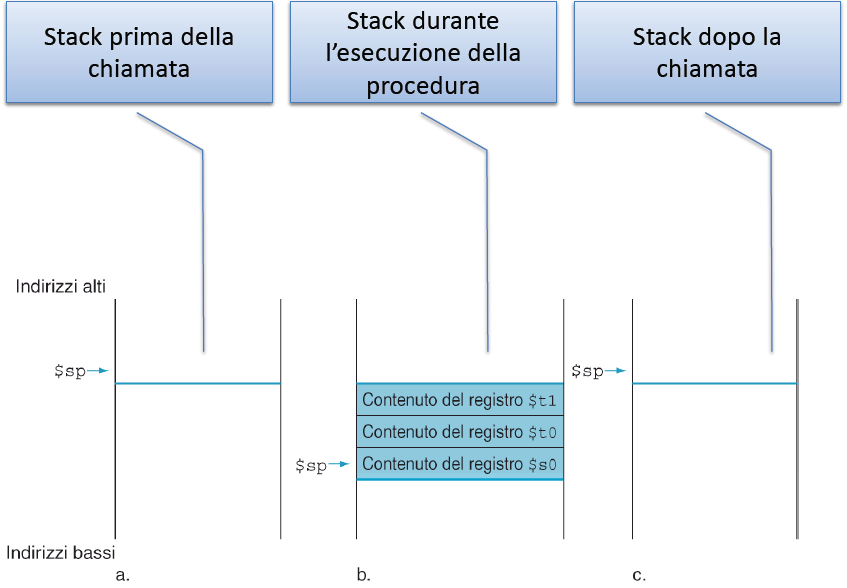
\includegraphics[width=0.8\textwidth,keepaspectratio]{Evoluzione-stack}
\end{figure}

Una volta visto l'esempio vanno fatte alcune precisazioni. Infatti un compilatore effettivo non avrebbe \emph{mai} svolto così la procedura, perché:
\begin{itemize}
	\item i registri temporanei \emph{non} devono essere preservati (quindi di norma non si usano istruzioni \mintinline{asm}{sw} e \mintinline{asm}{lw} su registri \emph{\$t...})
	\item l'utilizzo di \emph{\$s0} non era necessario (si poteva usare anche solo \emph{\$v0})
\end{itemize}

Vediamo ora un esempio più complesso, dove si affrontano ostacoli come variabili locali e procedure annidate (a detta di tutti temutissime); la soluzione che si applica in questo caso è di salvare nello stack appunto tutte le variabili locali e tutti i valori del registro \emph{\$ra} (per poi risalire la catena delle chiamate).

\begin{minted}[linenos, tabsize=4]{c}
int fact(int n){
	if (n < 1)
		return 1;
	else
		return n*fact(n-1);
}
\end{minted}

Si nota che implementando questa funzione il registro \emph{\$ra} ed il registro \emph{\$a0} vengano sovrascritti $n$ volte.
Vediamo quindi la traduzione del seguente esempio da C ad assembly MIPS:

\begin{minted}[linenos, tabsize = 4]{asm}
FACT:
	# decrementa $sp di 8 creando lo spazio per 2 words
	addi $sp, $sp, -8;

	# salva i registri $ra e $a0 nello stack
	# ricorda: $ra contiene l'indirizzo di ritorno post-funzione
	# ricorda: $a0 contiene il dato, in questo caso n
	sw $ra, 4($sp)
	sw $a0, 0($sp)

	# fine del prologo, inizio della procedura effettiva
	slti $t0, $a0, 1    # se $a0 < 1 setta $t0=1

	# $t0 settato a 1 se n < 1
	beq $t0, $zero, L1  # se $t0 == 0 si va a L1 (ricorsiva)

	# altrimenti si prosegue con l'esecuzione finale
	addi $v0, $zero, 1  # $v0 = 1
	addi $sp, $sp, 8    # si ripulisce lo stack

	# ritorna all’indirizzo dopo la chiamata (n-esima) di fact
	jr $ra
	# da questa istruzione parte la risalita della sequenza di $ra
L1:
	addi $a0, $a0, -1  # decrementa n
	jal fact           # chiama fact(n-1)

	# a questo punto si ripristina $a0 e $ra e si ripulisce lo stack
	lw $a0, 0($sp)    # ripristina $a0
	lw $ra, 4($sp)    # ripristina $ra
	addi $sp, $sp, 8  # ripulisce lo stack

	# infine moltiplica n*fact(n-1), che è in $v0, e ritorna
	mul $v0, $a0, $v0
	jr $ra
\end{minted}

\subsection{Gestione delle variabili in MIPS}
Le variabili in C sono in genere associate a locazioni di memoria e si caratterizzano per:
\begin{itemize}
	\item \emph{tipo}: (\mintinline{c}{int}, \mintinline{c}{char}, \mintinline{c}{float}, ecc.);
	\item \emph{storage class}:
	\begin{itemize}
		\item \emph{automatic}: variabili locali che hanno un ciclo di vita collegato alla funzione
		\item \emph{static}: variabili globali o statiche che sopravvivono anche al termine della funzione.
	\end{itemize}
\end{itemize}

Le variabili \emph{statiche} sono memorizzate in una zona di memoria specifica (nel MIPS accessibile attraverso il registro global pointer, \emph{\$gp}).

Le variabili \emph{automatiche} invece possono essere memorizzate nei registri, tuttavia quando questi non bastano, come già visto, le variabili vengono salvate all'interno dello stack; il segmento di stack che le contiene viene chiamato \emph{record di attivazione} (o \emph{stack frame}). Le variabili locali vengono individate tramite un offset a partire da un puntatore allo stack.\\
Contrariamente a come si penserebbe, non si utilizza \emph{\$sp} come puntatore, poiché esso può variare all'interno dello svolgimento di una funzione, di conseguenza si utilizza il puntatore dedicato \emph{\$fp}.

L'immagine qui sotto rappresenta l'evoluzione dei due puntatori \emph{\$sp} e \emph{\$fp} durante la chiamata di una funzione, per capire meglio i vantaggi dell'utilizo di \emph{\$fp}.
\begin{figure}[H]
	\centering
	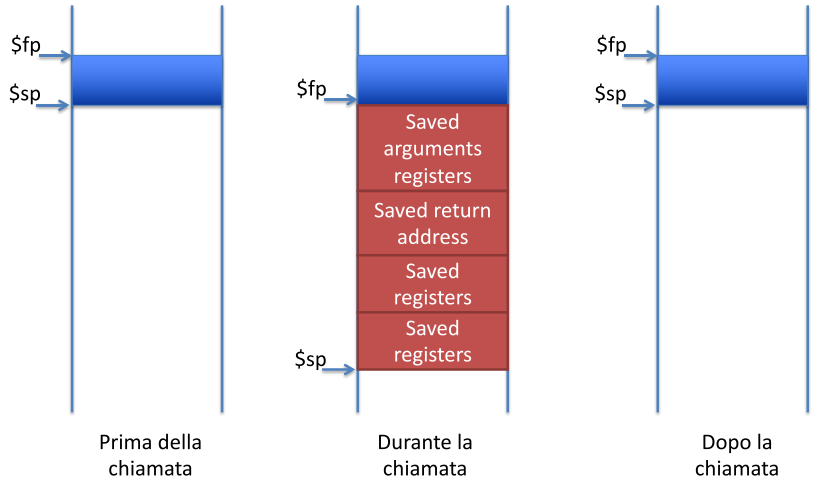
\includegraphics[width=0.85\textwidth,keepaspectratio]{sp-vs-fp}
	\caption{Confronto tra puntatore \emph{\$sp} e \emph{\$fp}}
\end{figure}

Esiste inoltre un ultimo tipo di variabili (oltre alle globali ed alle locali), quelle dinamiche, che vengono allocate secondo lo schema della figura sottostante dal MIPS; da notare il fatto che lo stack procede "decrescendo", mentre i dati allocati dinamicamente "crescono"  partendo da dove terminano i dati statici (e quindi si spiega perché negli esempi precedenti abbiamo decrementato \emph{\$sp} per inserire word nello stack).
\begin{figure}[H]
	\centering
	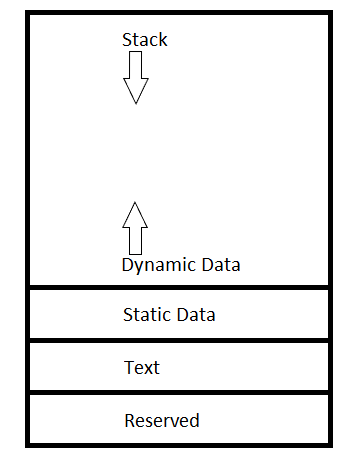
\includegraphics[width=0.4\textwidth,keepaspectratio]{Dove-finiscono-le-variabili}
	\caption{Schema allocazione dei dati in MIPS}
\end{figure}

\subsection{Elaborazione delle procedure}
Per spiegare come vengono elaborate le procedure complesse da MIPS utilizziamo come esempio la seguente funzione:

\begin{minted}[linenos, tabsize=4]{c}
int sum(int n){
	if (n > 0){
		return sum(n-1) + n;
	} else {
		return n;
	}
}
\end{minted}

Se si analizza la funzione si nota come il valore di ritorno viene costruito risalendo la catena di chiamate e quindi ogni frame di attivazione deve essere preservato per produrre il risultato corretto. Ecco come compare il codice assembly della procedura \emph{sum}:

\begin{minted}[linenos]{asm}
SUM:
	add  $v0, $a1, $zero   # sposta $a1 in $v0
	blez $a0, $L5          # se $a0<=0, salta a L5
	addi $sp, $sp, -32     # crea spazio nello stack
	sw   $ra, 28($sp)      # salva $ra
	add  $a1, $a1, $a0     # (acc = acc + n)
	addi $a0, $a0, -1      # (n = n - 1)
	jal  SUM               # ricorsione (aggiorna $ra)

	# parte di risalita della catena di $ra
	lw   $ra, 28($sp)      # ripristina $ra
	addi $sp, $sp, 32      # ripulisce lo stack
L5:
	j $ra                  # torna al programma chiamante
\end{minted}

Come possiamo immaginare il procedimento scritto così è  molto dispendioso in termini di memoria, ma possiamo, con un po' di esperienza e scaltrezza, riscrivere nel seguente modo il programma:

\begin{minted}[linenos, tabsize = 4]{c}
int sum(int n, int acc){
	if (n > 0){
		return sum(n-1, acc+n)
	} else {
		return acc;
	}
}
\end{minted}

In questo caso si applica il metodo di ricorsione in coda, che comporta un grande vantaggio dal punto di vista dell'utilizzo di memoria poiché una volta terminata una chiamata della funzione si può eliminare tutto il suo ambiente (che non risulterà più utile) e utilizzare sempre solo un ambiente unico ed un unico \emph{\$ra}, vediamo come:

\begin{minted}[linenos,breaklines]{asm}
SUM:
	add  $v0, $a1, $zero   # sposta $a1 in $v0
	blez $a0, $L5          # se $a0 <= 0, salta a L5

	add  $a1, $a1, $a0     # (acc = acc + n)
	addi $a0, $a0, -1      # (n = n - 1)
	j  SUM                 # ricorsione
	# si osservi come non si usa più jal dato che non si aggiorna più $ra ora che si lavora su un unico ambiente
L5:
	j $ra                  # torna al programma chiamante
\end{minted}
Alcuni compilatori sono in grado di ottimizzare automaticamente il programma in questo modo così da renderlo molto più veloce e leggero, il \mintinline{batch}{gcc} è in grado di aggiustare, ove possibile, questo tipo di procedure con una complessità pari a \emph{O(2)}.

\section{Le stringhe in MIPS}\label{sec:mipstring}
Nel linguaggio C le stringhe erano degli array di caratteri che terminava in \mintinline{c}{'\0'} (\mintinline{c}{NULL} character)
e, secondo la codifica ASCII, ogni carattere veniva codificato con un byte. Presentiamo qui una funzione che copia una stringa:
\begin{minted}[linenos, tabsize=4]{c}
void copia_stringa(char *d , const char *s){
	int i = 0;
	while((d[i] = s[i]) != 0){
		i+=1;
	}
}
\end{minted}
Appare chiaro che qui sovviene la necessità di copiare \emph{bytes}, non \emph{parole}. Vediamo quindi come implementare questa funzione in MIPS.

\subsubsection{Load byte e store byte}
Operare su byte anziché su parole intere può tornare utile anche in altre situazioni, per cui in MIPS disponiamo di istruzioni dedicate: \emph{load byte} e \emph{store byte}, analoghe a quelle che operano sulle words. Eccone un esempio:
\begin{minted}[linenos, breaklines]{asm}
lb $t0, 0($sp)  # leggi un byte dalla cima dello stack ed inseriscilo nei bit meno significativi di $t0

sb $t0, 0($gp)  # inserisci gli otto bit meno significativi di $t0 in $gp
\end{minted}

\subsection{Possibile implementazione}

\subsubsection{Prologo}
Come il lettore a questo punto saprà, i due parametri \mintinline{c}{d} e \mintinline{c}{s} sono contenuti in \emph{\$a0} e \emph{\$a1}. Supponiamo di voler utilizzare \emph{\$s0} per salvare il contatore \mintinline{c}{i} (anche se naturalmente un compilatore non lo farebbe \emph{mai}, lo salverebbe su un registro temporaneo). Il registro \emph{\$s0} andrà dunque salvato nello stack e successivamente inizializzato:
\begin{minted}[linenos, tabsize=4]{asm}
COPIA_STRINGA:
	addi $sp, $sp, -4      # crea spazio nello stack per salvare $s0
	sw $s0, 0($sp)         # salva $s0
	add $s0, $zero, $zero  # i = 0
\end{minted}

\subsubsection{Loop}
A questo punto procediamo all'implementazione del ciclo \emph{while} che eseguirà la copia di \mintinline{c}{s[i]} in \mintinline{c}{d[i]}. Iniziamo mettendo l'indirizzo di \mintinline{c}{s[i]} nel registro \emph{\$t1}.\\
(Nota: \mintinline{c}{&s[i] = s + i}, non \mintinline{c}{s + i * 4}).\\
A questo punto carichiamo \mintinline{c}{s[i]}
in \emph{\$t2} e salviamolo in \mintinline{c}{d[i]}.
\begin{minted}[linenos, tabsize=4, firstnumber=5]{asm}
L1:
	add $t1, $s0, $a1  # inizio loop
	lb $t2, 0($t1)
	add $t3, $s0, $a0  # metti (d+i) in $t3
	sb $t2, 0($t3)
\end{minted}
Ora che il corpo dell'istruzione è stato svolto, bisogna controllare se \mintinline{c}{s[i] == '\0'} e, in caso di risposta affermativa, il loop terminerà; altrimenti si incrementerà il contatore (che sta in \emph{\$s0}) e torna al ciclo.
\begin{minted}[linenos, tabsize=4, firstnumber=10]{asm}
	beq $t2, $zero, L2  # se la stringa è finita, vai a L2 e termina
	addi $s0, $s0, 1    # incrementa il contatore
	j L1                # torna al ciclo
\end{minted}

\subsubsection{Epilogo}
In questa fase viene implementata la fine del ciclo e il ritorno al chiamante; si recupera il valore precedente di \emph{\$s0}, viene ripristinato \emph{\$sp} e tutto ritorna.
\begin{minted}[linenos, tabsize=4, firstnumber=13]{asm}
L2:
	lw $s0, 0($sp)
	addi $sp, $sp, 4
	jr $ra
\end{minted}

\subsubsection{Mettendo insieme il tutto}
Ricapitolando, ecco come sarà la nostra procedura:
\begin{minted}[linenos, tabsize=4]{asm}
COPIA_STRINGA:
	addi $sp, $sp, -4
	sw $s0, 0($sp)
	add $s0, $zero, $zero
L1:
	add $t1, $s0, $a1
	lb $t2, 0($t1)
	add $t3, $s0, $a0
	sb $t2, 0($t3)
	beq $t2, $zero, L2
	addi $s0, $s0, 1
	j L1
L2:
	lw $s0, 0($sp)
	addi $sp, $sp, 4
	jr $ra
\end{minted}

\subsection{Implementazione realistica}
Nessun compilatore avrebbe mai lavorato in questo modo. Abbiamo presentato la procedura così affinché fosse didatticamente più efficace, adesso invitiamo il lettore a dare un'occhiata a quella che potrebbe essere la traduzione di un vero compilatore, in particolare \mintinline{batch}{gcc}:
\begin{minted}[linenos, tabsize=4]{asm}
COPIA_STRINGA:
	lb $v0, 0($a1)
	sb $v0, 0($a0)
	beq $v0, $zero, L5
	move $v0, $zero
L3:
	addiu $v0, $v0, 1
	addu $v1, $a1, $v0
	lb $v1, 0($v1)
	addu $a2, $a0, $v0
	sb $v1, 0($a2)
	bne $v1, $zero, L3
L5:
	jr $ra
\end{minted}

\end{document}
